% Made up for the tikra gallery: chemistry and commutative diagrams inside the drawing, which TikZ
% cannot nest (chemfig and tikz-cd are tikzpictures of their own); mathra sets them as math.
\documentclass[border=0pt]{standalone}
\usepackage{pgfplots}
\usetikzlibrary{backgrounds}
\definecolor{espresso}{HTML}{17100C}
\definecolor{crema}{HTML}{E8B87A}
\definecolor{caramel}{HTML}{C47A3A}
\definecolor{milk}{HTML}{F4E9DC}
\newcommand\mol[2]{$\chemfig{#1}$\\[3pt]\textcolor{crema}{\scshape #2}}
\begin{document}
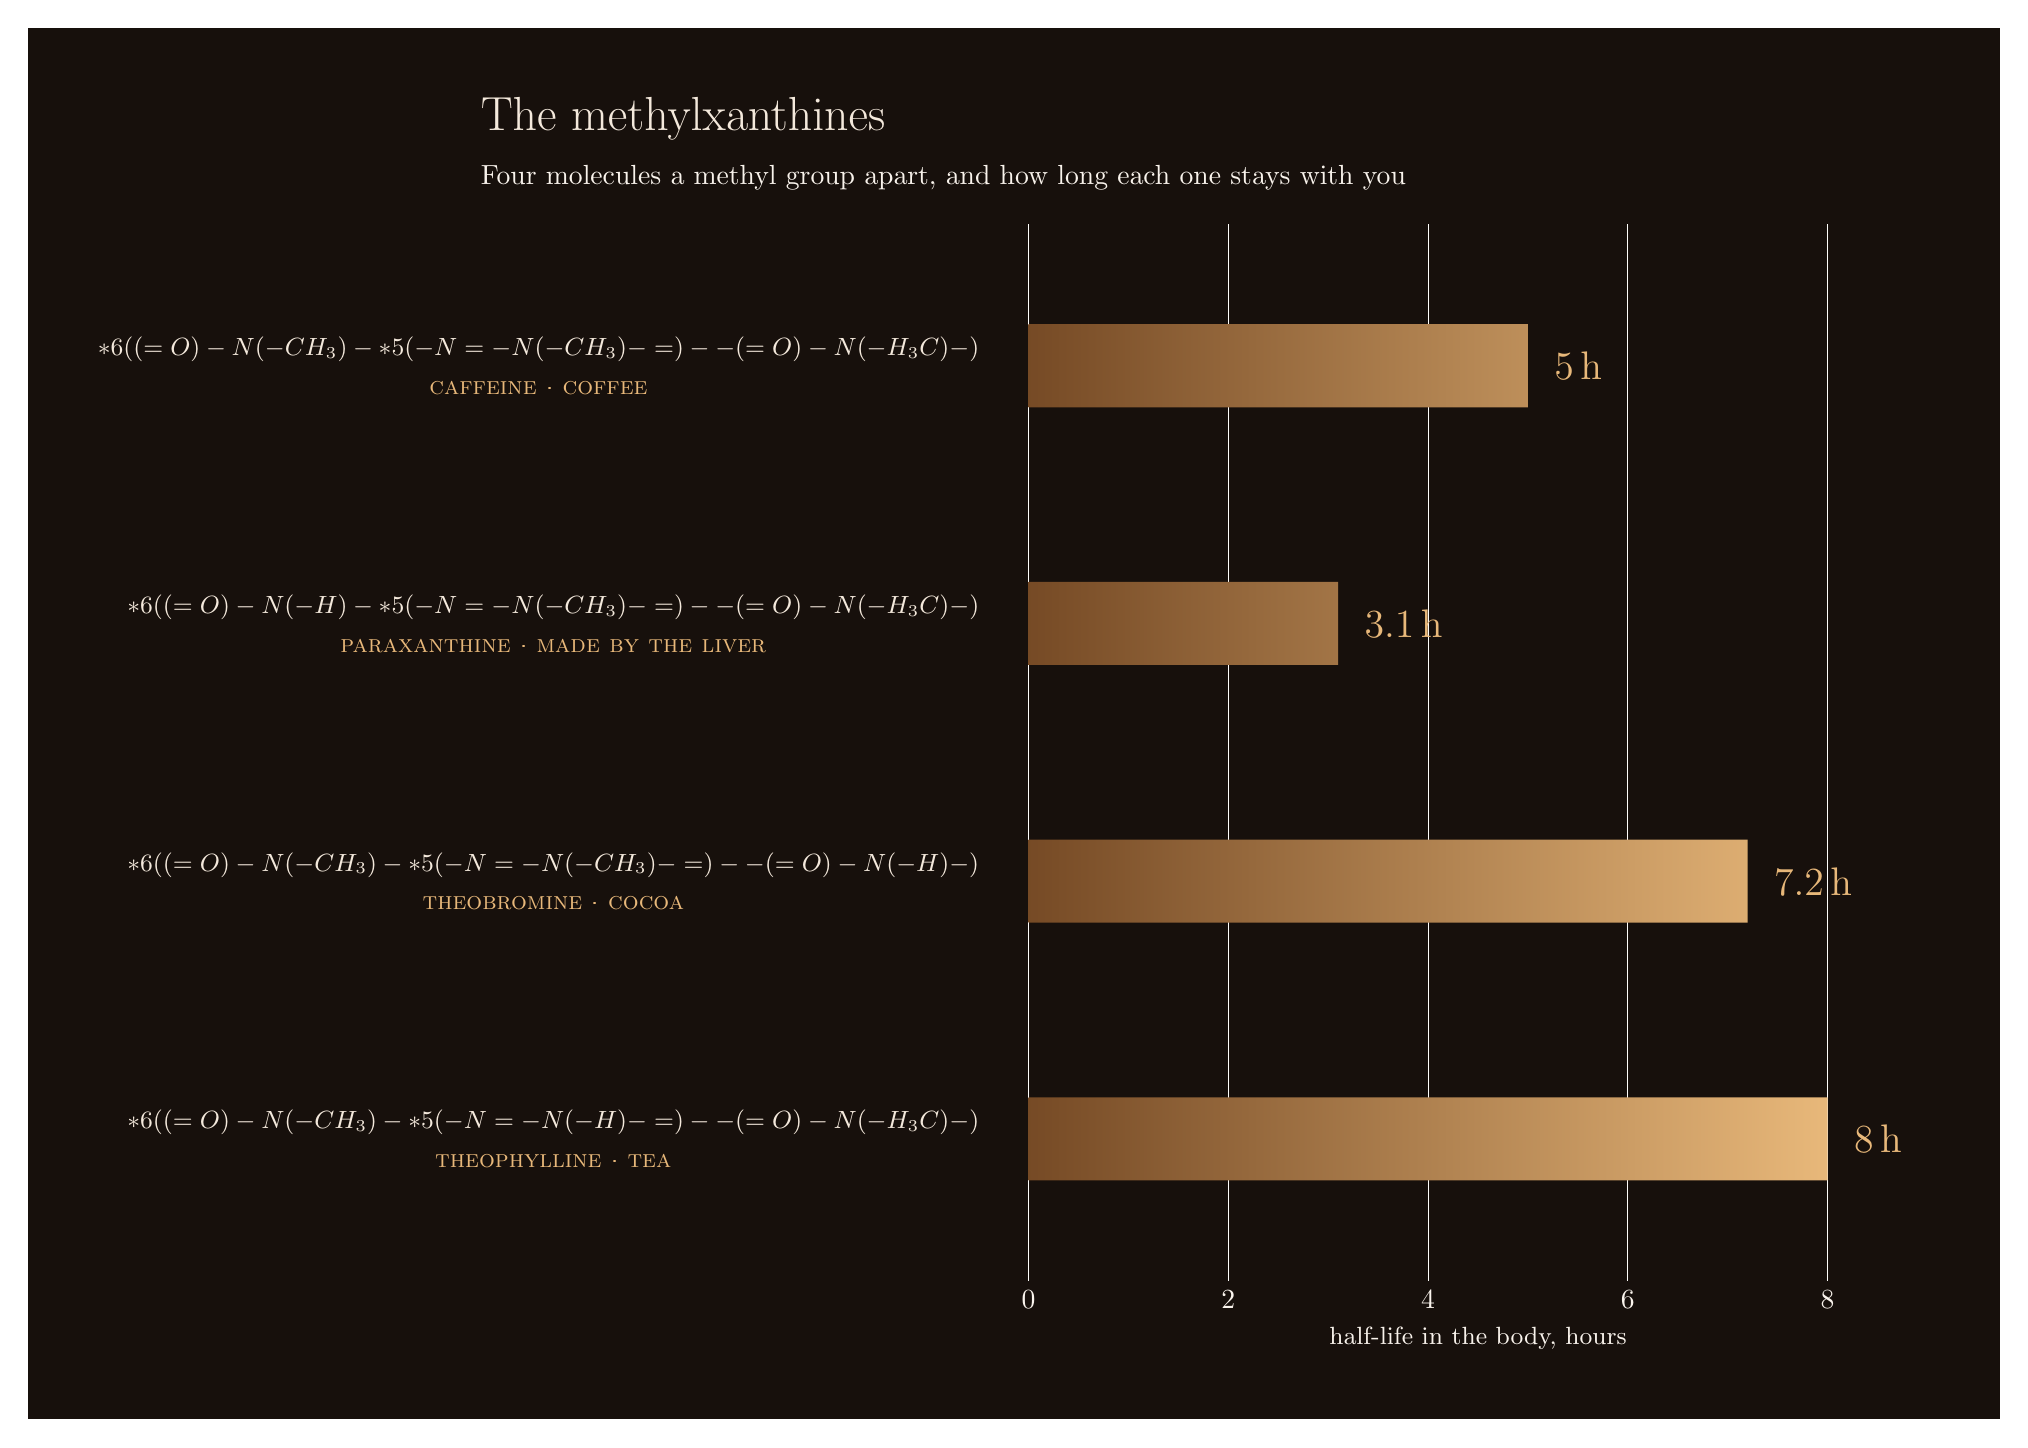
\begin{tikzpicture}[background rectangle/.style={fill=espresso, draw=none}, show background rectangle, inner frame sep=22pt]
\begin{axis}[
    xbar, bar width=30pt, width=13cm, height=15cm, clip=false,
    xmin=0, xmax=9, ymin=0.45, ymax=4.55,
    axis line style={draw=none}, tick style={draw=none},
    xmajorgrids, grid style={milk!10},
    xtick={0,2,4,6,8}, xticklabel style={text=milk!50},
    xlabel={half-life in the body, hours}, xlabel style={text=milk!55, font=\small},
    ytick={1,2,3,4},
    yticklabels={
      {\mol{*6((=O)-N(-CH_3)-*5(-N=-N(-H)-=)--(=O)-N(-H_3C)-)}{theophylline · tea}},
      {\mol{*6((=O)-N(-CH_3)-*5(-N=-N(-CH_3)-=)--(=O)-N(-H)-)}{theobromine · cocoa}},
      {\mol{*6((=O)-N(-H)-*5(-N=-N(-CH_3)-=)--(=O)-N(-H_3C)-)}{paraxanthine · made by the liver}},
      {\mol{*6((=O)-N(-CH_3)-*5(-N=-N(-CH_3)-=)--(=O)-N(-H_3C)-)}{caffeine · coffee}}},
    yticklabel style={text=milk, font=\small, align=center, xshift=-10pt},
    nodes near coords={\pgfmathprintnumber[fixed, precision=1]{\pgfplotspointmeta}\,h},
    nodes near coords style={text=crema, font=\Large, anchor=west, xshift=6pt},
    point meta=x,
  ]
  \addplot[draw=none, left color=caramel!55!espresso, right color=crema] coordinates
    {(8.0,1) (7.2,2) (3.1,3) (5.0,4)};
  \node[anchor=south west, text=milk, font=\LARGE] at (rel axis cs:-0.62,1.07) {The methylxanthines};
  \node[anchor=north west, text=milk!55] at (rel axis cs:-0.62,1.065) {Four molecules a methyl group apart, and how long each one stays with you};
\end{axis}
\end{tikzpicture}
\end{document}
